\documentclass[a4paper,12pt]{article}

\usepackage{fontspec}
\usepackage{xunicode}
\usepackage{textcomp}
\usepackage{graphicx}

\usepackage[english]{babel}

\usepackage{url}

\usepackage{colortbl}

\usepackage{subscript}

\usepackage{linguex}

\usepackage{qtree}

\usepackage{lscape}

\usepackage{longtable}

\usepackage{tabularx}

\setromanfont{Arial}

\usepackage{natbib}
\bibpunct[: ]{(}{)}{;}{a}{}{;}

\begin{document}

\tableofcontents
\newpage

\urlstyle{same}

\begin{flushleft}
\begin{Large}
\textit{Funding Initiative\\
\textbf{“Documentation of Endangered Languages”}}\\\bigskip
\end{Large}

\textbf{VolkswagenStiftung}\\
Dr.\,Vera Szőllősi-Brenig\\
Kastanienallee 35\\
30519 Hannover\\
GERMANY
\end{flushleft}

\begin{flushright}
\today
\end{flushright}

\begin{flushleft}
\begin{tabularx}{\textwidth}{ l | X }
\hline
\multicolumn{2}{>{\large\columncolor[gray]{0.8}} c }{Personal data and adresses}\\
\multicolumn{2}{>{\large\columncolor[gray]{0.8}} c }{Applicant(s), cooperation partner, grant recipient}\\
\hline
\multicolumn{2}{>{\large\columncolor[gray]{0.8}} l }{Principal applicant}\\
\hline
\hline
\textbf{Family Name} & {\textbf{Rießler}}\\
\hline
\textbf{First Name} & {\textbf{Michael}}\\
\hline
Female / Male & {Male}\\
\hline
Titel & {M.A. (Dr.\,phil expected 2010, thesis submitted July 2010)}\\
\hline
Field of Study & {Scandinavian linguistics}\\
\hline
\hline
\textbf{Institution} & \textbf{Albrecht-Ludwigs-Universität Freiburg i.\,Br.}\\
\hline
\textbf{Department} & \textbf{Skandinavisches Seminar}\\
\hline
Street & {Platz der Universität 3}\\
\hline
Postcode & {79085}\\
\hline
City & {Freiburg}\\
\hline
Country & {Germany}\\
\hline
Phone No & {+49-761-203-3300}\\
\hline
Mobile Phone No & {+49-179-9441585}\\
\hline
Fax No & {+49-761-203-3366}\\
\hline
E-Mail Address & {michael.riessler@skandinavistik.uni-freiburg.de}\\
\hline
Homepage & \url{www.skandinavistik.uni-freiburg.de/institut/mitarbeiter/riessler/}\\
\hline
\end{tabularx}
\end{flushleft}

\noindent The application has not been / will not be submitted to other funding institutions.\\

Signature\\

\noindent \textit{\textbf{Please note that the Volkswagen Foundation – in accordance with regulations safeguarding data privacy – records electronically your personal data as well as the project proposal.}}

\newpage

\begin{flushleft}
\begin{tabularx}{\textwidth}{ l | X }
\hline
\multicolumn{2}{>{\large\columncolor[gray]{0.8}} l }{Co-applicant}\\
\hline
\hline
\textbf{Family Name} & {\textbf{Trosterud}}\\
\hline
\textbf{First Name} & {\textbf{Trond}}\\
\hline
Female / Male & {Male}\\
\hline
Titel & {Ph.D.}\\
\hline
Field of Study & {Saami linguistics}\\
\hline
\hline
\textbf{Institution} & {\bf{Universitetet i Tromsø}}\\
\hline
\textbf{Department} & {\textbf{Institutt for språkvitskap}}\\
\hline
Postcode & {9037}\\
\hline
City & {Tromsø}\\
\hline
Country & {Norway}\\
\hline
Phone No & {+47-77644763}\\
\hline
E-Mail Address & {trond.trosterud@uit.no}\\
\hline
Homepage & {http://www.hum.uit.no/a/trond/}\\
\hline
\end{tabularx}
\end{flushleft}

\begin{flushleft}
\begin{tabularx}{\textwidth}{ l | X }
\hline
\multicolumn{2}{>{\large\columncolor[gray]{0.8}} l }{Co-applicant}\\
\hline
\textbf{Family Name} & {\textbf{Gerstenberger}}\\
\hline
\textbf{First Name} & {\textbf{Ciprian}}\\
\hline
Female / Male & {Male}\\
\hline
Field of Study & {Computational linguistics}\\
\hline
\hline
\textbf{Institution} & {\bf{Universitetet i Tromsø}}\\
\hline
\textbf{Department} & {\textbf{Institutt for språkvitskap}}\\
\hline
Postcode & {9037}\\
\hline
City & {Tromsø}\\
\hline
Country & {Norway}\\
\hline
%Phone No & {+47-77644746}\\
%\hline
E-Mail Address & {ciprian.gerstenberger@uit.no}\\
\hline
Homepage & {\url{http://www.hum.uit.no/a/gerstenberger}}\\
\hline
\end{tabularx}
\end{flushleft}

\begin{flushleft}
\begin{tabularx}{\textwidth}{ l | X }
\hline
\multicolumn{2}{>{\large\columncolor[gray]{0.8}} l }{Co-applicant}\\
\hline
\textbf{Family Name} & {\textbf{Wilbur}}\\
\hline
\textbf{First Name} & {\textbf{Joshua Karl}}\\
\hline
Female / Male & {Male}\\
\hline
Field of Study & {Documentary Linguistics}\\
\hline
\hline
\textbf{Institution} & {\bf{Humboldt-Universität zu Berlin}}\\
\hline
\textbf{Department} & {\textbf{Nordeuropa-Institut}}\\
\hline
Postcode & {10099}\\
\hline
City & {Berlin}\\
\hline
Country & {Germany}\\
\hline
%Phone No & {+49-30-2093-4850}\\
%\hline
E-Mail Address & {wilburjk@staff.hu-berlin.de}\\
\hline
Homepage & {\url{http://www.ni.hu-berlin.de/personal/jwil/jwil_html}}\\
\hline
\end{tabularx}
\end{flushleft}

\newpage

\section*{Project proposal}

\section{Basic information}

\begin{tabbing}
LLLLLLLLinks \= Mitte \= Rechts \kill
Title: \>\textbf{Language Technology for Small Saami Languages}\\
Budget: \>\textbf{€ 298,822}\\
Period: \>\textbf{August 2011 – July 2014}\\
\end{tabbing}
\begin{flushleft}
Keywords: {\it Documentary Linguistics, Saami Linguistics, Computational Linguistics, Applied Linguistics, Corpus Linguistics, Revitalization; Kildin Saami, Ter Saami, Pite Saami, Ume Saami, ISO 639-3: sjd, sjt, sje, sju}
\end{flushleft}

\section{Abstract} 
The proposed project will use existing DoBeS and ELAR archives to create a state-of-the-art corpus infrastructure as well as language technology tools for four endangered Saami languages: Ume, Pite, Kildin and Ter Saami. This shall involve a variety of aspects relevant to the field of modern documentary linguistics: endangered language documentation and archiving practices, automatic annotation, and computer-aided tools for creating lexica and educational materials. Ultimately, the project intends to develop new methods for processing already extant archived linguistic data from endangered Saami languages in order to improve subsequent/future corpus linguistic research and to support language revitalization efforts with language technology.

The main goal of the project is twofold: 1) to apply language technology tools to efficiently supplement corpora of digitized, transliterated and translated texts with consistent annotations, and 2) using the resulting annotated corpora, to then create practical applications such as paradigm and word-form generators, interactive teaching materials and electronic lexica. As a result, the needs of both the academic community and the speech communities concerned will be served.

Specifically, the project shall result in the following outcomes: 1) a searchable corpus of spoken language for these four endangered Saami languages which shall be linked to multimedia files and intended not only for use in linguistic research, but also as a gateway to the corpus for the language communities; 2) semi-automatic annotation of the corpus; 3) implementing language tools for both linguists and revitalization activists such as lemmatizers, part-of-speech taggers, dependency parsers, (online/offline) electronic dictionaries, translation tools, educational materials, etc.; 4) development of methods, workflows, conventions and best-practice guidelines for such projects; and
5) dissemination of these outcomes to be utilized in the future as at least a template or source of inspiration for other DoBeS, ELAR and other endangered language projects for developing corpus linguistics and language technologies.

Pite Saami and Ume Saami are spoken in Sweden, while Kildin Saami and Ter Saami are spoken in Russia; they belong genealogically to distinct subbranches of the Saami group inside Uralic: Ume is in the southern branch of West-Saami, Pite in the central branch of West-Saami, and Kildin and Ter belong to the Peninsula branch of East-Saami. All four languages are highly endangered or moribund due to ongoing language shift to the regional suprastrate Indo-European languages Swedish and Russian.

For three of the four languages in question, annotated multimedia corpora already exist thanks to the groundwork carried out by principle applicant Michael Rießler (partially with the help of co-applicants E.\,Karvovskaya and J.\,Wilbur) for the Kola Saami Documentation Project (a DoBeS project) and by co-applicant J.\,Wilbur for the Pite Saami Documentation Project (a Hans Rausing Endangered Languages Project). These corpora covering Kildin, Ter and Pite Saami will form the initial core set of resources for the project's work, but will be supplemented with more data and more elaborate annotations in the course of the project, as well as with addition of the first annotated corpus of Ume language materials. While automatic generation of annotations and corpora is nothing new, the application of such computer-aided technologies to spoken, multimedia archived materials of endangered languages is a first.

Community-driven revitalization efforts are underway to varying extents for all four languages. Thus, there is local interest in working on these languages while speakers are still living, and the proposed project will work closely with the language communities in producing practical products in tune with the respective communities' wishes and expectations.

The project will be carried out within the framework of contemporary documentary linguistics and as a joint effort between the Scandinavian Department at Freiburg University and the center for Saami language technology (Giellatekno) at the University of Tromsø.
The team shall consist of experienced documentary and computational linguists as well as programmers, all of whom are familiar with Saami languages in general and have excellent working knowledge of the Saami languages in question and the relevant \textit{lingua franca}. Team members are also well versed in corpus- and computational linguistics, in carrying out documentation fieldwork, and in practical revitalization issues. The project will also profit from the symbioses already in place between researchers familiar with the Giellatekno infrastructure (including tools for other northern languages) and researchers acquainted with the DoBeS and ELAR infrastructures (documentary linguistics of spoken language, archiving of annotated multimedia).

The two leaders of the project are documentary linguist Michael Rießler (Freiburg) and computational linguist Trond Trosterud (Tromsø), both of whom are specialized in Saami linguistics. The first applicant is a junior researcher who also led a DoBeS project on the Kola Saami languages. The other two applicants are Joshua Wilbur, currently coordinator/researcher for the Pite Saami Documentation Project (ELDP), and Giellatekno's programmer Ciprian Gerstenberger. Funding for the proposed project would go towards a full principle researcher position for M.\,Rießler and a half-time principle researcher position for J.\,Wilbur at the University of Freiburg, two student research assistants as well as material support and travel expenditures.

\begin{figure}[h]
\begin{center}
\caption{S\'{a}pmi and the Saami languages. The languages of the project are shaded.} 
\label{SaamiLgs}
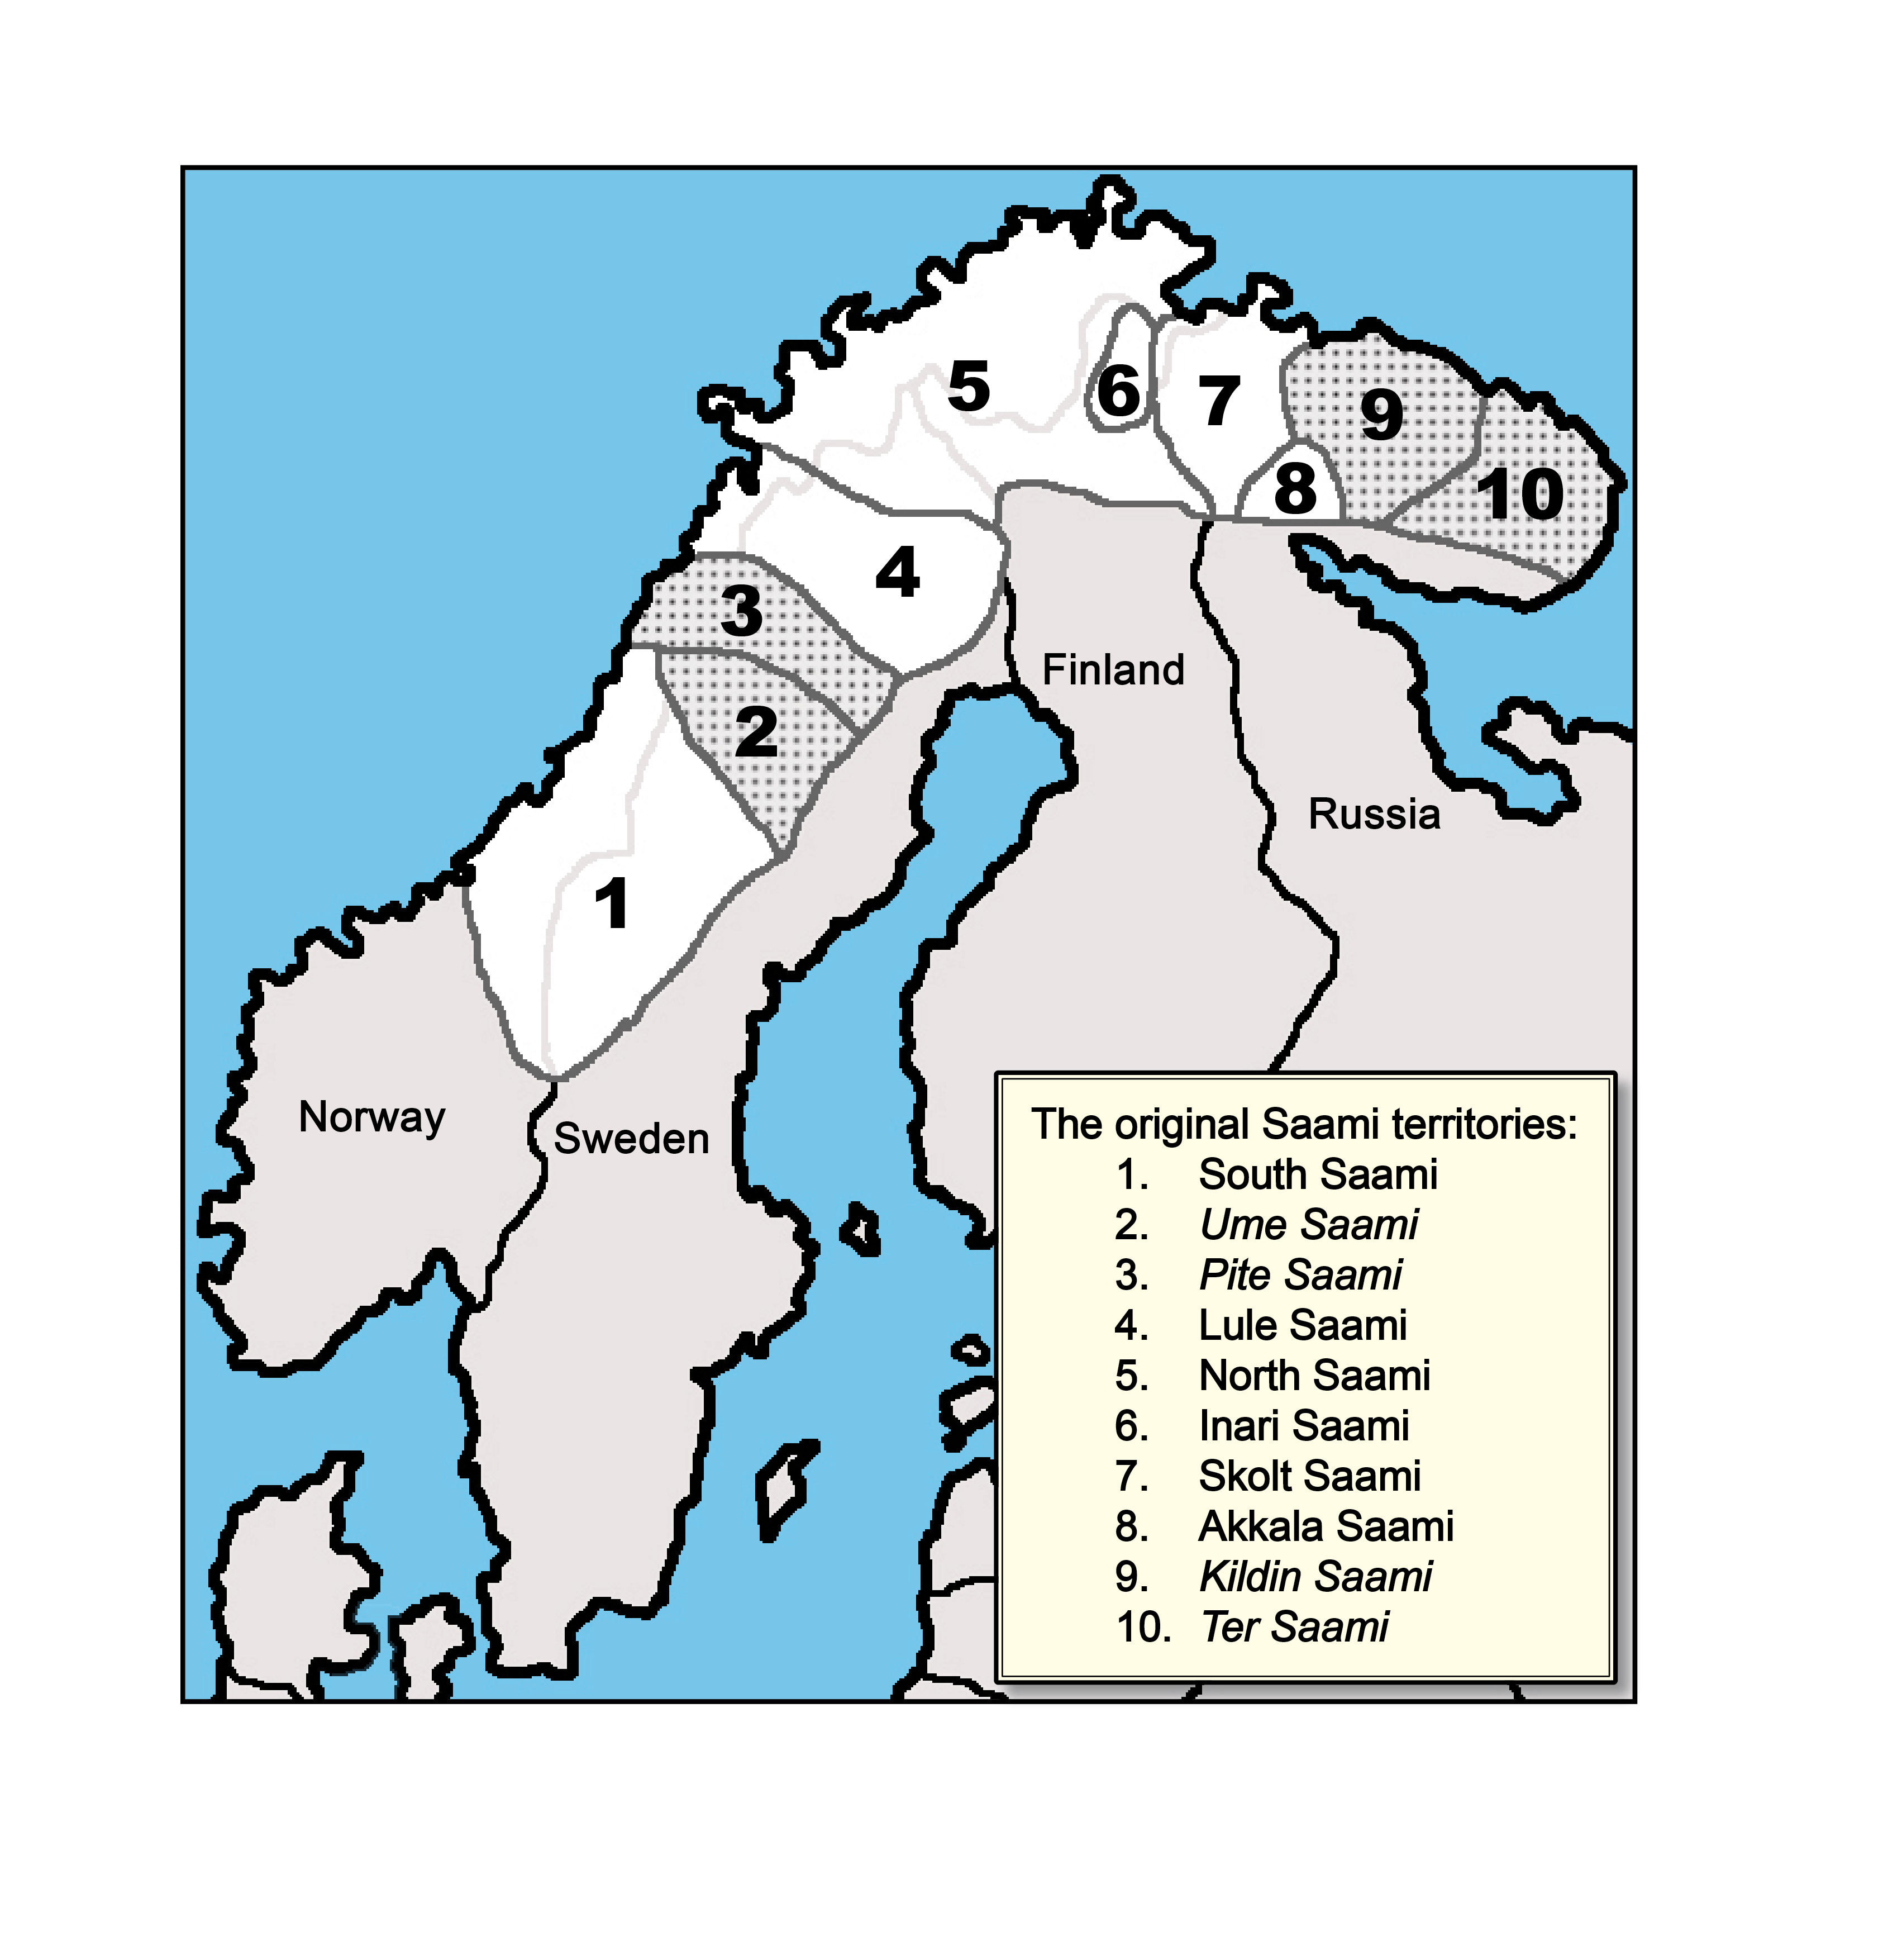
\includegraphics[width=0.9\textwidth]{SaamiLgs.jpeg}
\end{center}
\end{figure}

\section{Detailed project description}
\subsection{Introduction}

The \textit{Dokumentation bedrohter Sprachen} (DoBeS) and the \textit{Hans Rausing Endangered Language Project} (which ELAR is a part of) programs have the aim to create data-orientated, multifunctional, and generally accessible documentations of endangered languages in order to support languages in danger of extinction and to help protect endangered linguistic and other cultural data from disappearing. In this, archiving recordings of spoken languages alone is not considered sufficient; instead, archived recordings must include metadata and annotations describing their contents. This should at least consist of cataloging metadata (concerning e.g. participants, recording location, etc.) and transcriptions of the recordings with translations into a stable \textit{lingua franca}. However, annotations can provide much more detailed information, such as the specifics provided by detailed linguistic analyses\footnote{Detailed linguistic analyses typically contain such information as part of speech, glosses, and/or word or morpheme boundaries.}. Such analyses are interesting and useful in and of themselves for linguistics research, but they also can be utilized to produce lexica, translation tools and teaching materials for use by linguists and, at least as important, by the relevant endangered language community. However, producing such detailed analyses is exceptionally time and resource consuming, and as a result, only a portion of archived materials typically include such detailed information. Fortunately, with the help of current computer-based technology, the availability of such detailed linguistic analyses in a computer-readable format can result in:
\begin{itemize}
\item easier and more effective searches of documentation corpora for both corpus linguists and language community members, including linking search results to the actual primary recordings;
\item the creation of lexica, translation tools and educational materials utilizing modern web-based technologies.
\end{itemize}
It is thus the logical next step from the perspective of both language and research communities to supplement archived materials with as much detailed linguistic analyses as possible and then, with the help of computers, to create practical products as a result. This task is particularly urgent for endangered languages because 1) access to native speaker knowledge is limited and potentially no longer possible in a relatively short time, and 2) because those involved in revitalization efforts want to take advantage of the practical tools that result in counteracting wide-spread language death at a local level as soon as these become available.

\subsection{Preliminary considerations}
\paragraph{What are corpora?} In principle, any collection of language data is a corpus. However, raw, i.e. unannotated, data is normally processed and annotated according to the purpose of data collection. This means that all transcriptions of recorded texts result in a kind of searchable corpora. If at least one translation is provided with the transcription, then it is considered to be a parallel corpus. Most Saami language documentation work is currently available as parallel corpora in books or other printed media, but is thus only searchable manually. If such text corpora are scanned using text-recognition software (OCR, Optical Character Recognition), they can then be made machine-readable, but the results can still only be used for raw text searches. In accordance with the central aims of contemporary documentary linguistics, i.e. data orientation, multi-functionality and general accessibility, DoBeS corpora (similar to ELAR or other archives) do not only provide a direct link to the original recordings but in most cases these corpora also include independent linguistic (and even other non-linguistic) annotation. Normally, these annotations are created as the result of tedious manual labour or by using semi-automatic (morphological) parsers like Toolbox.

For languages with good access to informants or even native linguists, there is always the possibility of introspection and informant elicitation when collecting data, but this includes running the risk of being influenced by the research situation. Ideally, corpus data are gathered independently of the linguistic problem at hand, and therefore are an example of genuine language use. Nonetheless, corpus data face methodological problems: corpora are problematic when investigating non-existent and marginal forms, yet for endangered, let alone extinct languages, corpus studies are the only empirical foundation available. In order to enable also future generations to investigate the languages in question, large and diverse corpora are needed.

\paragraph{What is corpus linguistics?} Corpus linguistics refers to the study of linguistic phenomena as expressed in real world texts such as in the printed text representations mentioned above, or in machine-readable corpora, which allow for much more efficient corpus research. One significant problem when trying to create a “quality” machine-readable corpus is keeping annotation standards consistent; this includes reserving one type of information for each annotation tier (e.g. part-of-speech in one tier, glosses in another tier), consistent use of certain tags or symbols for similar phenomena (e.g. sticking to a set list of morphological glosses, to a set method of morpheme boundaries, defined marking of non-linguistic phenomena, etc.). As opposed to strictly manual annotations, which are mistake-prone, semi-automatic annotation methods using software such as Toolbox allow for more consistent tagging, at least in theory. However, in practice, some corpora stemming from Toolbox projects are only really searchable using a full text search due to inconsistent tagging and including several different kinds of information (e.g. phonological, morphological and morpho-phonological) into one and the same annotation tier. As a result, searching the content of such corpora is relatively limited.

A further problem with annotating and tagging transcriptions manually is the simple fact that this is exceptionally time consuming, as is evidenced by the fairly small amount of detailed annotation relative to the total number of transcriptions for archived language materials. Computer-aided annotation, on the other hand, provides a significantly faster and more efficient way to provide detailed annotations to a transcription.

To allow for multi-layered, consistent annotation of linguistic data, the use of off-the-shelf and open-source annotation tools (e.g., NITE XML, MMAX, UAM CorpusTool, etc.) is indispensable. However, the idiosyncratic socio-cultural development of each Saami language poses challenges for building language corpora and making them work with annotation and searching tools. To choose and adapt such annotation tools for languages with peculiar writing systems, e.g. Kildin, is not a trivial task. The present project aims at choosing and adapting such tools for the appropriate language representation for the languages under discussion. All tools developed by the project will be open-source and freely available for adaptation by other language technology projects. 

\paragraph{What are computational linguistics and language technology?} Computational linguistics refers to machine-based processing of natural language. This normally includes, among other things, the development of processes for the analysis and generation of natural language texts, programs to collect and statistically evaluate large amounts of language data (such as lemmatizing software, frequency wordlists, concordances). Computational linguistics also eases the process of building corpora mostly by using automated processes (typically morphological and syntactic disambiguation). A further goal for computational linguists is to build models of natural language grammars. When tested against actual language data, such models function as hypotheses for the structure of the grammar in question. 

Language technology could be considered to be a (functional) application of computational linguistics as it is aimed at analyzing and generating natural language in various ways and for a variety of mostly practical purposes. Machine-based translation or computer-based language instruction are two examples of such practical applications.
 
\paragraph{What are multimedia spoken vs. written corpora?}
The Giellatekno group in Tromsø already has the know-how and the infrastructure necessary to deal with the above aspects of corpus and computational linguistics, and has fully implemented this for North Saami, as well as partly for Lule Saami and South Saami, and has even completed some initial work for Kildin Saami. However, these are all written languages and the text corpora which Giellatekno's work has been based on have also been in written form (as mono-lingual or parallel texts with translations). The proposed project intends to take advantage of Giellatekno's experience and expand its field of application exclusively to spoken corpora. In theory, the input for the computational linguistic applications will be the same, since the spoken texts will first have to be represented as text (ortho-)graphically. However, there are several important aspects to consider in this (cf.~below Section \ref{method}).

Furthermore, many corpora are exclusively represented in writing, including the existing Giellatekno corpora. The proposed project, in focusing on spoken-language texts, will include links to the time-aligned multimedia recordings that the orthographic representations which make the corpora originate from. In and of itself, this is also nothing new. However, the corpora resulting from the proposed project will be linked to multimedia sources and include annotations done by semi-automatic morphological and syntactic parsing. In this, we will be joining documentary linguistics on endangered languages with corpus linguistics and with language technology. It is precisely these considerations which are at the source of motivation for the proposed project. As such, one of our main goal is to create a corpus linguistic infrastructure as a foundation for future Saami linguistic work using the DoBeS and ELAR materials. The other main goal being practical tools for aiding revitalization.

\paragraph{Why specifically these four Saami languages?}
There are a variety of reasons why precisely these four Saami languages have been chosen as the focus of the project. First of all, the depth and detail of annotations for archived endangered language materials for these Saami languages will be expanded. Second, the work going into creating automatic parsing tools will also be used to create practical language tools, which in turn will support current revitalization efforts by the respective language communities. Third, it is both sensible and practical to adapt Giellatekno experiences with North Saami\footnote{Specifically, this includes the computational linguistic infrastructure which is already in place for written North Saami as well as the computational linguistic know-how derived from dealing with monolingual and parallel written North Saami corpora.} to related Saami languages rather than starting from scratch. Fourth, these four Saami languages display interesting variation between each other in regard to both the quantity and quality of their respective documentation resources as well as to the degree to which they are written; such variation allows for complex and rewarding methodological comparisons. Last but not least, the tools, workflows, experience and guidelines resulting from the project shall be able to be used as a kind of example or template for other projects working with language technology and/or corpora of endangered spoken languages.

\subsection{Urgency of documentation}\label{urgency}
The Saami languages (Uralic) form a dialect continuum across an area extending from central Scandinavia to the Kola Peninsula in the Russian Federation. Traditionally, the Saami were half-nomadic peoples who migrated annually between summer and winter settlements and survived on hunting and fishing. Herding reindeer was not a typical occupation until relatively recent times, but has become so at least in the central mountainous areas of Sápmi; nowadays all Saami live modern lives and blend in with the rest of the predominantly non-Saami population. Due to the influence of North Germanic, Finnic and Russian languages and cultures, all ethnic Saami are fluent in their respective contact languages, while younger generations are typically monolingual in these. As a result, the Saami languages are today either extinct, moribund or endangered. The least endangered Saami language is North Saami with not more than 17,000 speakers in Norway, Sweden and Finland \citep[1]{sammallahti1998b}.

\begin{figure}
\caption{Saami language tree} \label{saami tree}
\qtreecenterfalse
\Tree [.Saami [.{West Saami} [.South South Ume ] [.Central Pite Lule North ] ] [.{East Saami} [.Mainland Inari Skolt ✝Akkala ] [.Peninsula Kildin Ter ] ] ]
\end{figure}

The proposed project will focus on four particularly endangered Saami languages, as summarized here:
\begin{itemize}
\item Kildin (highly endangered, with an orthography, with some description and documentation)
\item Pite (moribund, without an [established] orthography, with little description and documentation)
\item Ter (moribund, without any orthography, with little description and documentation)
\item Ume (practically extinct, without an [established] orthography, with very little description and documentation)
\end{itemize}

Ume is a southern Saami language of West-Saami and spoken in central Swedish Lapland in and around the modern towns of Arvidsjaur, Malå, Ammarnäs and Tärna. Today, Ume is practically extinct, as the estimated number of speakers is less than five.\footnote{This is co-applicant J.\,Wilbur's own estimate, based partly on hear-say, and consists of one elderly woman in Lycksele, one man (approx. 40 years old) who taught himself Ume as a second language, but speaks it with his two children, who could be considered Ume speakers; according to J.\,Wilbur's contacts in Arjeplog, there are also two or three elderly non-active speakers in Arvidsjaur, Sweden.} Although the first Saami language book ever was a new testament bible translation in Ume Saami from 1755, no standardized orthography has been developed, nor is there any significant set of literature in Ume. However, one Ume language activist has recently developed some educational materials and texts on his own.

The situation for Pite Saami is not quite as desperate, but can hardly be described as positive. Pite (also known as Arjeplog Saami) is in the central branch of West-Saami and is currently spoken by approximately 30 speakers in and around the community of Arjeplog in central Swedish Lapland. Of these speakers, the vast majority are 50 years old or older and have neglected to teach their children Pite. There is one exception, a 33 year old reindeer herder who actively speaks Pite on a daily basis in his work with his family's reindeer, and speaks Pite with his two young sons (6 and 4 years old). As with Ume, Pite does not have an established orthography; however the local Saami association in Arjeplog is currently completing a project called \textit{Insamling av pitesamiska ord}\footnote{Expected completion in December 2010.} to collect a wordlist consisting of several thousand words, and is creating an orthography in the process. Co-applicant J.\,Wilbur has worked closely with the project as an unofficial “linguistics consultant” and in many conversations with Nils-Henrik Bengtsson, the project coordinator, has heard about the project's interest in using the wordlist to create a dictionary and pedagogical materials.

Historically, Ume and Pite were also spoken in the adjacent parts of central Norway, but today, the territory in which they are spoken has been reduced to a small area in Swedish Lapland due to repressive language policies in both Norway and Sweden, particularly during the first half of the 20\textsuperscript{th} century. Today, Swedish language and culture dominate the lives of the Ume and Pite Saami to such an extent that their languages have practically been wiped off the map due to language shift to Swedish. Indeed, \citet[123]{blokland-etal2003} point out that Swedish laws protecting the status of Saami minorities lag behind those in Norway and Finland; this has contributed to a faster decline of Saami languages and culture in Sweden. Current Swedish (and Norwegian) language legislation only applies to South, Lule and North Saami, and ignores Ume and Pite as separate languages \cite[180]{seurujarvi-kari2005}, despite the fact that they are considered independent languages by linguists \citep[cf.][]{sammallahti1998b,salminen2007}. Even a recent language law introduced in Sweden in 2009 and intended to protect and support minority languages only recognizes Saami as one single language, despite the significant linguistic and social divides between the various Saami groups. Effectively, the other three Saami languages spoken in Sweden (North, Lule and South Saami), but particularly North Saami (with the most robust group of speakers in Sweden, Norway and Finland, as well as with radio and television support) block any chances that Ume or Pite might have for gaining public recognition. 

While knowledge of Pite lexical items is common particularly among reindeer herders, the language is rarely used as a means of communication. No classes are taught in school, not even as a foreign language, however there have been sporadic intensive courses over the last two decades, targeted mostly at teaching reading and writing using the Lule Saami orthography.

Ter and Kildin Saami spoken in Russia together form the Peninsula branch of East-Saami. Ter is nearly extinct and spoken by no more than 30 speakers or semi- speakers living in different locations within and outside of the Murmansk region, such as in Murmansk, Lovozero, Gremicha, Revda, Krasnoščel'e, Umba, and also in Saint Petersburg. The mean age of the youngest speakers of Ter is over 50. Kildin is actively spoken by no more than 100 native speakers \citep{scheller2010}, though the number of passive speakers is surely much higher and comes perhaps to 700. However, the number of speakers is decreasing rapidly from year to year. The language is no longer passed on to children and must be characterized as severely endangered.

Originally, Kildin was spoken in the central inland parts and the central coastal parts of the Kola Peninsula. The original Kildin dialect areas have fragmented chiefly as the result of forced centralization. Today, more or less compact Kildin Saami settlements in or close to their original villages are found only in Lovozero, Revda, Kola, Loparskaja and Teriberka, but small Kildin Saami speech communities are also found today in all larger towns, such as in Murmansk, Olenegorsk, Apatity, etc. As a result of the forced resettlement of most of the Kola Saami population to Lovozero, this village is nowadays usually regarded as the ‘Saami capital’ of Russia, and in fact Lovozero has by far the densest Saami population today. However, less than a third of the village’s approximately 3000 inhabitants are ethnic Saami, and the number of Saami speakers among these is considerably lower.

Kildin is the only actively used Kola Saami language today. It is also the only standardized Saami language of Russia. Since most Kildin Saami speakers live in Lovozero, the central and probably most innovative variety of this former Saami settlement has been chosen as a normative basis for the language is usually being regarded as the Kildin Saami standard. The current Cyrillic-based orthography for Kildin was developed during the 1980s, and since then different kinds of teaching materials for elementary schools and school dictionaries using some variant of this orthography have been published. Even though Kildin is standardized, the language is used neither in official business or administration nor as a medium of education. In mass media, Kildin is only marginally represented. Radio programs in Kildin have been broadcast locally  in Lovozero since 1983, but broadcasting time has never exceeded 5–20 minutes per day. Some fictional literature in Kildin has been published in books and journals, but these texts consist almost exclusively of short tales and poems for children or translations into Kildin Saami. At present, Kildin is taught to children only in one school in Lovozero. This weekly course is optional and for grades 1 through 4 only. One pre-school in Lovozero has a Saami group in Kildin. Besides that, classes in Kildin are occasionally taught for children and adults at different places in the region.

In addition to the fact that all four Saami languages considered here are in desperate need of documentation and that revitalization seems unlikely at present (despite an increase in interest among younger ethnic Saami) for Pite, Ter and Ume from a purely linguistic point of view, they prove to be interesting both cross-linguistically and within Saami studies. Unlike the other Indo-European languages in the area, Saami languages are almost exclusively suffixing and predominantly have postpositions. Phrases are generally head-final, although SVO has become grammatical as well, just as postponed relative constructions occur. Saami case systems consist of between seven and nine cases. Verbs and pronouns are inflected for singular, dual and plural number categories (not in Kildin and Ter). In all four investigated languages, all inflectional case suffixes have been retained, and accusative and genitive cases are still differentiated morphologically; they are thus considered more archaic than other Saami languages to the north and east that have lost some case endings and have come to lack an accusative-genitive distinction.

Additionally, Saami languages are known for their complicated non-linear morphology realized as ablaut, umlaut, consonant gradation (phonological alternations in a stem's consonants triggered by the morphological environment) and/or palatalization of noun and verb stems (in Kildin and Ter and also in Skolt). In general, regressive vowel harmony (umlaut) in Saami languages is found in the initial stressed syllable of a stem with its allophone being adjusted to the vowel in the second and unstressed syllable. Pite is especially interesting in this respect because it has progressive vowel harmony concerning lip rounding in the same environment \cite[272]{korhonen2005a}. Ume is interesting because it has a large variety of umlauts and the least amount of consonant gradation, with the exception of neighboring South Saami, the only Saami language lacking consonant gradation. Whether proto-Saami also had consonant gradation is a controversial issue \cite[cf.][154–55]{svonni2006}, and further information about this phenomenon in Ume and Pite could help inform this debate. Furthermore, Ume is unique among Saami languages in having trisyllabic stems in the nominative case \cite[421]{korhonen2005b}; the role nonlinear morphology plays in words of this length is unclear. Moreover, the linguistic topics of information structure and focus have been almost completely neglected in Saami linguistics in the past.

The resulting corpus from the proposed project could help Saami linguistics to come to a more detailed understanding of these topics and these specific Saami languages' places in Saami studies and linguistics in general. Finally, completion of such elaborately detailed corpora will be an asset for corpus linguistics and provide more date for future research in morphology, syntax and lexicology by both Saami and general linguists on these and other topics.

\subsection{State of research}
\subsubsection{Language documentation}

The languages under consideration are not completely undocumented; in fact, for three of the four languages in question, annotated multimedia corpora already exist thanks to the groundwork carried out by principle applicant M.\,Rießler (partially with the help of co-applicants E.\,Karvovskaya and J.\,Wilbur) for the Kola Saami Documentation Project \cite[a DoBeS project, cf.][]{KSDP} and by co-applicant J.\,Wilbur for the Pite Saami Documentation Project \cite[a Hans Rausing Endangered Languages Project, cf.][]{PSDP}.

Within the course of the Kola Saami Documentation Project (the archive will be completed by December 2010), recordings of both Kildin and Ter Saami were collected, transcribed and partially annotated for archiving at DoBeS, and are thus available through the DoBeS archive. M.\,Rießler and L.\,Karvovskaya have worked extensively on these languages and will be able to continue programming the morphological and syntactic automators which have already been initiated within the Giellatekno framework. All text-based digital resources found in the DoBeS archive, including the Kildin and Ter recordings and annotations, can be searched efficiently with the help of corpus tools developed by the Technical Group at the Max-Planck Institute for Psycholinguistics in Nijmegen, the Netherlands, where the main DoBeS servers are located (cf.~Section \ref{dobesTools}).

Other audio recording for Kildin and Ter are stored at archives in Helsinki, Tallinn and Petrozavodsk. They are all archived with only a minimum of metadata; any further annotations are lacking, with the exception of a handful of texts from the Petrozavodsk archive for which some written transcriptions and translations have been published in \citealt{kert1961} and \citealt{panfilov-etal1988}. There are also a few older text collections for Kildin and Ter available for which recordings are not available at all. For Kildin, a comprehensive (but outdated) descriptive grammar can be found in \citealt{kert1971}. A descriptive grammar for Ter has been produced as an (unpublished) Ph.D. dissertation \cite{tereskin2002a}\footnote{unfortunately this grammar is essentially useless because for the most part it simply copies Kert's 1971 Kildin grammar and misses a number of important Ter features, not to mention the many inconsistencies and frequent typos.}. A comprehensive (but outdated) descriptive dictionary of all Kola Saami dialects is provided by \citealt{itkonen_t_i1958a}, while \citealt{kuruc-etal1985} and \citealt{kert1986} are school dictionaries for Kildin.

Some linguistic work has been done on Pite in the past. Juhani Lehtiranta published a Pite grammar in Finnish in \citeyear{lehtiranta1992}, but in fact this grammar is based on earlier studies done between 1890 and 1950, and thus does not necessarily reflect current usage. There is also an old Pite grammar in German from \citeyear{lagercrantz1926} written by Eliel Lagercrantz. There is no dictionary of Pite.

Aside from discussions of Pite in a few various articles, that was essentially the extent of linguistic work on this language. However, due to the Pite Saami Documentation Project, various papers and talks have been presented or are underway, and a Ph.D. dissertation including a sketch grammar and a description of morpho-phonological phenomena shall also be completed by the end of 2012 by co-applicant J.\,Wilbur. Even more significantly, the project is still in the process of collecting, transcribing/translating and partially annotating recordings for archiving. In August 2010, the first Pite materials went online at the Endangered Languages Archive (ELAR) in London. This initial deposit consists of six audio/video recordings and the respective ELAN annotation files, as well as related images and metadata definition files. These recordings cover a variety of genres (from descriptions of traditional handicrafts and reindeer herding practices, reindeer vocabulary, and everyday conversations). As the project will be concluded in July 2011, more recordings and transcriptions/annotations will be deposited and made available online\footnote{Access to archived materials is only available to registered users and each file may have even more limiting permission levels; however, at this point, all files are at least available to the Pite Saami community members and the linguistic research community}, including elicitation sessions, in the near future. These Pite materials can be accessed via the ELAR website at \url{www.hrelp.org/archive/} (cf. also~Section \ref{elarTools}).

As a Pite sketch grammar will be included in co-applicant J.\,Wilbur's Ph.D. project, and his knowledge of and experience with Pite Saami and previous work with Giellatekno will allow him to program morphological and syntactic automators.

In addition to the Pite resources mentioned above, there are also a number of Pite legacy recordings at the archive of the Dialekt-, ortnams- och folkminnesarkivet i Umeå (DAUM)\footnote{\url{www.sofi.se/daum/}}, however these are completely without transcriptions, translations or other annotations, are only partially digitized and are archived with a minimum of poorly searchable cataloging metadata.

Ume is by far the most endangered among the Saami languages considered here, as it has likely a maximum of five living speakers. Some work has been done on Ume in the past, the most significantly of which is an Ume-German dictionary based on the speech of the village Malå (a dialect which is now extinct) published by Wolfgang Schlachter in \citeyear{schlachter1958}. In 1738 a dictionary and the only grammar of Ume appeared \cite{fjellstrom1738a,fjellstrom1738b}.
As with Pite, there are some legacy materials for Ume at DAUM, but these are also lacking any transcriptions, translations or other annotations, are only partially digitized and are archived with a minimum of poorly searchable cataloging metadata. However, J.\,Wilbur has received permission to access these materials in supplement them with transcriptions and further annotations.
Despite the exceptionally small number of speakers, there is also some revitalization activity underway within the Ume ethnic community, and Peter Steggo (one of the project's external specialists) has recently been appointed the official municipal language consultant for the Ume Saami community of Arvidsjaur.

It should also be noted that there is a considerably larger amount of material (texts, dictionaries, annotated recordings and linguistic work)  available for Lule and South Saami (the two neighboring languages to the north and south), which can prove useful in understanding and analyzing both Pite and Ume data.

\subsubsection{Corpus search tools at DoBeS/MPI}\label{dobesTools}
All tools are available free of charge and with an open-source license, and the Technical Group intends to continue maintaining these tools into the foreseeable future, ensuring accessibility to archived data to future generations of linguists and speech community members; even if support for the tools should cease to exist, archived files are written as simple text in the open format XML, which is both readable by both machines and humans\footnote{While considered to be readable by humans, more complicated XML files are not necessarily a pleasure to read for the layperson.}. These tools are available online via the Language Archiving Technology website at \url{www.lat-mpi.eu}. The usefulness of these tools for the intents of the proposed project are summarized below.
\begin{itemize}
\item ELAN (EUDICO Linguistic Annotator) allows audio and video recordings to be time aligned with detailed transcriptions, translations and further annotations. Because ELAN permits one to link digital text-based annotations with the actual recordings of linguistic events themselves, it is the platform on which the project's corpora will be based. ELAN files are simple text files written in XML, a current archiving standard because it is an open format which is machine and (somewhat) human readable. Elaborate searching, including use of regular expressions, is possible within a single ELAN file or across several files, all stored on a local computer or network; search results can be shown in a \textit{key-words in context (KWIC)} format, in other words, a context of up to eight words on either side of the search term are visible; and a complex multiple-layer search limiting the context of neighboring tiers can also be performed (same software/GUI as with ANNEX/TROVA); finally, search results can be saved.
\item IMDI-Browser (ISLE Metadata Initiative Browser) is a web-based interface which allows one to search throughout the MPI corpora, including the DoBeS resources. With this browser, cataloging metadata as well as transcriptions, translations and other annotations can be searched in. Using the same software and graphic user interface as in ELAN, a multiple layer search can also be performed and results can also be organized in a KWIC format; finally, search results can be downloaded and saved.
\item ANNEX/TROVA is the software and graphic user interface behind the search engines mentioned above for ELAN and the IMDI-browser. However, a complex linguistic search across archived materials using the IMDI-Browser is unfortunately not very feasible because most of the data is only translated and lacking grammatical or more detailed linguistic analysis, and even the detailed linguistic data present in the various annotations has used a variety of different annotation conventions. Partially in an attempt to increase inter-searchability between the proposed project's annotations and other annotations in the MPI corpora, but also in following good documentation practices, the project will create and document transparent glossing practices based on accepted conventions, such as those described in the Leipzig glossing rules\footnote{\url{www.eva.mpg.de/lingua/resources/glossing-rules.php}}. Due to the very nature of automatic annotation, all project transcriptions are guaranteed to be glossed consistently.
\end{itemize}

\subsubsection{Corpus search tools at ELAR}\label{elarTools}
The first ELAR resources from a variety of HRELP-funded projects went online in summer 2010, and at this point, searching through ELAR materials online is limited to a character-string searches of basic cataloging metadata for a single project's deposits only\footnote{While the ELAR search capabilities are still quite limited, the ability to filter archive resources by participant or given keywords reflects ELAR's prioritizing of user-friendliness, particularly concerning non-linguist users from language communities. ELAR is planning to increase the complexity of search options in the future.}. However, all Pite Saami recordings archived at ELAR include annotations in ELAN and are thus in a format which is searchable using the available Language Archiving Technology tools mentioned above in section \ref{dobesTools}. To achieve the Pite Saami outcomes for the project, copies of these ELAN files will then be stored on the DoBeS/MPI servers to allow these to be searched as well, and, in cooperation with ELAR\footnote{David Nathan, the director of ELAN, has has indicated his interest in discussing and working on possibilities for the project to access ELAR materials.}, the respective audio and video materials at ELAR will be virtually connected to the DoBeS archive to allow linking of search results to multimedia. While the intention in this is to design a way to link up multimedia files between independent archives, if this in fact proves to be more complicated than valuable for the project, then copies of the relevant Pite multimedia files will be stored in the DoBeS archive.

\subsubsection{The Saami language technology project}

The language technology project Giellatekno\footnote{\textit{Giellatekno} is North Saami and means “language technology”.} already has an infrastructure setup for building language analyzers for several Scandinavian and other northern languages. This infrastructure has been set up for Pite and Kildin Saami, and for both languages there is an embryonic analyzer, containing some items from each part of speech, and some of the basic morphological and morphophonological processes for nouns and verbs. The Kildin Saami analyzer has also been included on the Giellatekno home page, cf. \url{http://giellatekno.uit.no/cgi/index.sjd.eng.html}.  No language technology work has been done for Ume or Ter Saami yet.

For South, Lule and North Saami a wide range of analyzers and applications are available. The best investigated language is North Saami, for which there are a morphological analyzer/generator, a syntactic analyzer, including grammatical functions and dependency; morphologically enriched dictionary, machine translation systems, a system for automatic phonetic transcription, and an interactive language learning program suite (\url{http://oahpa.uit.no}) including processing and feedback on free user input. With the relevant basic grammatical resources in place, similar programs may also be developed for the other Saami languages, including the languages of the present application (cf.~the following Section \ref{aimsmethod}).

\subsection{Research aims and methodologies}\label{method}
\subsubsection{General}%rather finished, last paragraph on Ume needs a check - urgent!

In addition to its general aim of contributing to the documentation and revitalization of endangered languages, the project will work within the framework of the following three main areas: 1) formal linguistic description (morphology and syntax as basis for parser creation), 2) computational linguistics (creation of parsers), and 3) programming (creation of lexica and other tools). The main goal of the project is twofold: 1) to apply language technology tools (more precisely: finite-state transducers and constraint grammar) to efficiently supplement DoBeS and ELAR multimedia corpora of digitized, transliterated and translated texts with consistent annotations, and 2) using the resulting annotated corpora, to then create practical applications such as paradigm and word-form generators, interactive teaching materials and electronic lexica. 

A number of interesting general issues concerning methodology will arise in working on four languages with differing (documentary) linguistic situations. These include: how to best deal with annotations of spoken language for corpus linguistics, how to deal with shortcomings in standard orthographies and orthographic variation, etc. In this respect, the project will also prove valuable for future research by contributing its experience and ideas to the general discourse on such topics. As a result, the needs of both the academic community and the Saami speech communities concerned will be served. Furthermore, the workflows and tools developed in the course of the project will enrich general methodology in Documentary Linguistics, especially since the results can be useful for other documentation projects specifically aimed at the creation of better corpus linguistic infrastructures and practical applications for endangered spoken languages.

One significant difference between this project and common practice in DoBeS and other documentation projects is that we will only annotate the orthographic representations and turn these into results useable by corpus linguistics. Otherwise, no practical products (such as dictionaries and teaching materials) would result. On the other hand, most other documentation projects create morphological annotations using a phonological transcription or an orthography based on phonemic principles (frequently created by researchers themselves); while such annotations can be quite precise, they require a lot of time and leave much room for inconsistencies and mistakes.

In our project, we will use identical principles for a variety of Saami languages, which can then theoretically be expanded for both other Saami languages and other languages around the globe. A further advantage will be that our corpora of spoken language can later be merged with written language corpora (at least for Kildin there are now a good number of written texts) and the tools developed in the project should work equally well for written language. And of course, the annotations that are created automatically based on the orthography will be aligned with the original recordings in the DoBeS and ELAR archives. In line with the main policies of DoBeS, and indeed documentary linguistics in general, the project supports linguistics oriented towards actual recorded data, as well as the data's multifunctionality and general accessibility, thus allowing other researchers to supplement annotations as they see fit, e.g. with morpheme breaks, phonetic annotations, etc.

After preparing, cleaning up and unifying the relevant text corpora, the main focus will be on programming analyzers and generators. Once these are in place, a wide range of possibilities opens up for language analysis and development. Linguistic analysis will benefit from lemmatization and grammatical analyses: from a given corpus of collected texts, analyzers may keep track of which lemmata are covered in a dictionary and which are not. For revitalization work, initial wordlists can be produced, and the analyzers may form the backbone of pedagogical programs.

Given the different quantity and quality of their documentation, the degree of successful revitalization efforts inside their speaker communities (including the existence of established orthographies) and the existence of previous language technology work, the project will devote its time and resources to the four languages to various extents: from the creation of a basic corpus and language technological infrastructure for Ume Saami to a full range of representative corpora and tools for Kildin Saami.

Generally, we can build on Giellatekno's already existing and functioning infrastructure and tools for written North Saami (and partly also for other written Saami languages). With the help of Giellatekno's experience and know-how, the project will start working with Kildin Saami, which has an established orthography, some successful revitalization efforts, the most available documentation is available and which already has a small corpora and a few limited tools at Giellatekno.

The biggest challenge for using the extant North Saami tools for Kildin, aside from reprogramming for different morphological and syntactic systems and a different script (Cyrillic), is establishing useful and consistent annotation conventions for phenomena specific for spoken text.

Once a sufficiently large Kildin test corpus has been created and morphological parsing is running successfully, we will approach Pite in a similar way. Giellatekno's existing resources for North Saami and especially for closely related Lule Saami will make it easier to program parsers for Pite. However, Pite Saami has a smaller amount of transcribed text recordings available (as compared to Kildin). Furthermore, there is no established orthography, at least not at the time of writing; however, there is a group of local Pite Saami activists currently developing an orthography\footnote{This project is called {\it Insamling av pitesamiska ord} and is being carried out by the local Saami association in Arjeplog the leader of which is one of the project's external specialists; co-applicant J.\,Wilbur is working closely with the project as a linguistics consultant. See section \ref{urgency} for more.}, and their preliminary orthography will be used, but this may have to be amended later once a standard has been agreed upon.

At the same time, we will continue to work on Kildin Saami and begin testing syntactic parsing operations.

As with Pite, there is no established orthography for Ter Saami, but the amount of available transcribed texts is even smaller than for Pite.  On the other hand, Ter Saami is very closely related to Kildin and the Kildin morphological and syntactic parsers can probably be easily adapted for use with Ter.

Finally, Ume currently has no orthography, practically no documentation, and is linguistically relatively distant to Pite (and the other Saami languages). As a result, we are only planning 1) to create a rather small corpus of transcribed, translated and annotated text; and 2) to write a morphological parser. The transcription and annotation data we will create will supplement the Schlachter corpus of Ume Saami text, for which transcriptions and translations are already available in digital form\footnote{Cf.~\url{the Schlachter corpus is stored at the UHLCS site in Helsinki http://www.ling.helsinki.fi/uhlcs/readme-all/README-uralic-lgs.html#C32}, 
and also at DAUM. %??? 
The texts were collected, transcribed, and published by Wolfgang Schlachter, and later digitalized and morphologically annotated by Olavi Korhonen. It includes 109,572 words, 561,654 characters (including tags); character encoding is ISO 8859-1 (Latin-1).}. This corpus first will aid in processing 
%the exclusively spoken data % include this formulation if we know that DAUM has more Korhonen data than the Schlachter ones
possible % ??? remove if we know they are different
other Ume recordings collected by Olavi Korhonen and archived at DAUM. 
 and provide a significant digital collection of lexical items. These recordings first have to be aligned in ELAN before 
further annotations will be done. % the thing is that the corpus unfortunately is presented in UHLCS as follows: "The morphologically analyzed and tagged Ume Saami corpus is a preliminary version of the Ume Saami text corpus compiled and encoded by Olavi Korhonen. The texts, which are told by Lars Sjulsson, Malå, Sweden, are based on the data recorded by Olavi Korhonen". But upon closer inspection of the data, the person Lars Sjulsson told his stories to, was Schlachter, and the man who wrote them down and published them, was again Schlachter (in Waldlappos. Upon closer inspection of the UHLCS presentation (cited above), one finds that it, very strictly speaking, does not contradict the textual findings. 
% What we need to know is whether there in DAUM is Ume data by Korhonen __in addition to__ the Schlachter data or not.

\subsubsection{Language technology}

Currently, the dominating paradigm within language technology is based upon statistical methods, upon teaching the computer the behavior of natural language by means of presenting it for vast amount of either un-analyzed or manually analyzed data. This approach achieves results superior to the most common grammar-based approaches. For the majority of the world's languages, and especially for the Saami languages treated here, this approach is not a viable option. The amounts of text needed – analyzed or not – is simply not available. The competing paradigm is grammar-based analysis: The researcher writes a machine-readable version of the grammar, and compiles into a program capable of analyzing and eventually also generating text. Several grammatical schools work within the grammar-based paradigm, the approached chosen by Giellatekno, and also by the present project, is a combination of using finite-state transducers for the morphological analysis and generation, and constraint grammar for disambiguation and syntactic analysis. This approach routinously gives better results than all competing paradigms, has been applied successfully by Giellatekno for (written) North Saami and which is therefore also chosen here.

Giellatekno's approach (finite-state transducers and constraint grammar) differs from most grammar-based systems in that it gives robust analyses for unconstrained text input. This is especially important for languages with complex morphology, and for spoken language, often consisting of long and repetitive sentences with opaque syntactic structures.

\paragraph{Segmental morphology}
For the morphology Giellatekno uses a compiler for modeling stems, segmental affixes and their grammatical analyses into a finite state transducer. The grammars are written within the $lexc$ formalism, and compiled with either the \texttt{lexc} or the open source \texttt{hlexc} compilers. 

The upper side of the resulting transducer consists, for each wordform, of a lemma and a string of grammatical tags, and the lower side is the concatenation of stem, affixes and markers signaling suprasegmental rules. The lower side of the $lexc$ transducer is fed to the Two-Level-Morphology component.

\paragraph{Two-Level-Morphology}
The suprasegmental morphology of Saami will be handled by the so-called Two-Level Morphology (TWOL). In TWOL, suprasegmental processes are handled not as serial rules, but as a transition between two levels:
\begin{description}
\item[on the upper side, the morphological/lexical level] root, affixes, affix borders, markers indicating suprasegmental processes (this corresponds to the lower side of the segmental transducer
\item[on the lower side, the morphographic level] the surface realization of the wordform
\end{description}
The two-way mapping between the two levels is mediated through a set of language-specific two-level rule. The compilation process results in a morphophonological TWOL parser.

For the Saami languages in question, important TWOL rule sets include the ones needed to model process such as consonant gradation, vowel harmony and diphthong simplification. The segmental transducer and the TWOL transducer are composed into one transducers, with lemma and grammatical tags on the upper side, and the corresponding wordform on the lower side. The transducer may be inverted, and it can both analyze and generate wordforms.

The composition of these two different transducers makes it possible to handle languages with rich morphological systems as complex as the Saami ones. 

\textit{Giellatekno} uses transducers made by TWOL and $lexc$ %JW: $lexc$ doesn't show up in my pdf!
in order to make language technology applications such as pedagogical programs, spell checkers, and programs for linguistic analyses. The programs are available for several Saami languages, and even for Greenlandic, Faroese, Komi and other languages.

\paragraph{Constraint grammar for syntactic analysis}
For disambiguation and syntactic analysis, Giellatekno uses \textit{Constraint Grammar} (CG). CG takes morphologically analyzed text as input, and returns only the appropriate readings, enriched with grammatical functions and dependency relations. The output may also be converted to phrase structure representation.

\paragraph{Parallel corpora}
Our Pite and Kola Elan files include in fact parallel corpora because the Saami texts are translated consequently with two languages: Pite-Swedish-English and Kildin/Ter-Russian-English resp. Parallel corpora are important for several purposes:
\begin{itemize}
\item Word-aligned corpora serve as input to multi-lingual dictionaries and term collections
\item Sentence-aligned text is a good starting point for writing contrastive grammars or as resource for
Computer-Aided Translation (CAT) tools 
\item To the extent that the corpora are big enough, they might also reveal statistical tendencies
\end{itemize}

\subsubsection{Methodological challenges}
On the one hand, the project will use annotation and presentation tools (ELAN and LEXUS) as well as corpus tools (like ANNEX/TROVA) created by the Language Archiving Technology team. These tools have been created specifically to meet the needs of quite divergent linguistic and anthropological documentation projects. In this, it is crucial, and in accordance with current methods in Documentary Linguistics, that annotations are linked to multimedia, discoverable via rich metadata and accessible via user-friendly interfaces.

On the other hand, the project will benefit from methodologies and language technology created by Giellatekno specifically for written Saami languages (though they have also been successfully applied to other (written) languages). The existing Giellatekno written corpora are thus of a very different character, particularly because they are not linked to multimedia and do not necessarily represent spoken language.

Several methodological considerations arise from combining a documentary linguistic approach (in this case DoBeS) and a corpus and computational linguistic approach (in this case Giellatekno). Confounding the situation is the fact that possessing a digital corpus and having a user-friendly interface for presenting and exploring the data do not necessarily go hand in hand. 

Fortunately, the ELAN and ANNEX/TROVA programs present corpus data with a relatively easy to learn graphic user interface while allowing for complex searches both on a local computer or network and online in the entire DoBeS/MPI archive, respectively. However, the transcribed, translated and annotated DoBeS/MPI language archive data do not, in the narrow sense, truly form corpora (in the sense of corpus linguistics), but are instead an irregular collection of multi-tier annotations with a maximum of both linguistic and non-linguistic information. However, to effectively search for a certain phenomenon, these annotations need to be refined and made consistent first. Furthermore, in practice, only a portion of archived recordings are provided with anything more than transcriptions and translations because of the simple unfortunate fact that time and manpower are usually insufficient to manually annotate everything.

To tackle this situation, our project intends to combine corpus linguistics and documentary linguistics in a sensible way: We plan to use documentations (with multimedia and transcriptions/translations) to create automatic linguistic annotations (for morphology and, partly, for syntax) in order to then efficiently make large corpora available; the resulting annotations will be linked to the original multimedia language resources, resulting in data which is more valuable for both ourselves and other researchers. And on top of that, we will produce language tools as a sort of “byproducts”, which are then useful for both researchers and for the language communities and revitalization activities.

The solution to these questions will thus not only be crucial to our project, but will also be relevant for other linguistic undertakings, particularly for documentary linguists interested in improving their documentation for use in corpus linguistics, and for corpus linguists involved in collecting data from spoken and/or endangered languages.

\paragraph{Corpora of standard written languages vs. corpora of spoken endangered languages} 
Very large corpora of written languages are available. Corpora of spoken languages (e.g., dialects or sociolects of written languages) are also commonly used in linguistic research, but such corpora are normally much smaller. The formal difference between corpora for written and spoken languages is mostly an issue regarding conventions on how spoken text is represented in written form. Spoken language is normally characterized by phenomena such as hesitations, false starts and self-corrections, which have to be dealt with in the annotations. Furthermore, the linguistic units are different, as spoken language cannot be divided into sentences. Annotators of corpora of endangered spoken languages, finally, have additional problems caused mostly by the typically high linguistic variation due to language attrition and language loss as well as code-switchings to contact languages.

Lists of spoken language annotation conventions already exist, such as those from projects which attempt to include as much information as possible; see for instance the conventions suggested by \citealt{schulze-bernd2006} specifically for documentary linguistics. For the proposed project however, it is more prudent to develop more of a “minimalist” catalogue of sensible annotation conventions with our project in mind. Anyone interested in studying spoken language will of course be able to use our ELAN files and add to these whatever information and annotations they desire.

\paragraph{Orthography issues}
Because we will be working with the orthographic representation of spoken language data and we are producing practical tools for language users, we will have to deal with orthography issues in the course of the project. As it is now, Kildin has an established orthography, but this has several variants. A first Pite orthography is currently under development by community members in collaboration with J.\,Wilbur; a working version is already being used in the Pite Saami Documentation Project. Ter Saami is lacking an orthography, but could use the Kildin orthography fairly easily; however, community members must decide to do so first. For Ume, the situation is still unclear. We will also be faced with orthography issues such as how to deal with variants and possible changes originating from inside the communities.

In solving these issues, we will work closely with the respective language communities while remaining objective and scientific, particularly since orthography matters can be the subject of much political controversy. Fortunately, the Giellatekno approach is able to deal with variations without forcing standardization, as evidenced by the way that the two main North Saami orthographies are both recognized by Giellatekno tools.

\subsection{Expected outcome of the proposed project}
In summary, the project shall result in the following general outcomes:
\begin{itemize}
\item a searchable corpus of spoken language for these four endangered Saami languages which shall be linked to multimedia files and intended not only for use in linguistic research, but also as a gateway to the actual language materials for the language communities;
\item semi-automatic annotation of the corpus (part of speech, morphology, syntax, gloss);
\item creation of language technology tools for both linguists and revitalization activists such as lemmatizers, intelligent dictionaries, translation tools, educational materials, etc.; 
\item development of methods, workflows, conventions and best-practice guidelines for such projects;
\item dissemination of these outcomes to be utilized in the future as at least an example or a source of inspiration for other endangered language projects developing corpus linguistics and language technologies.
\end{itemize}
We consider it self-evident that the resulting products will be free, open-source, open-access and platform-independent. These outcomes are described in more detail in the following (sections \ref{projectResult1} through \ref{projectResult3}).

\subsubsection{Project results: Corpus linguistics}\label{projectResult1}
\paragraph{Searchable, consistently and completely annotated multimedia Saami corpora at DoBeS/ELAR}
All Kildin, Ter and Pite texts from the DoBeS and ELAR archives will be parsed with detailed linguistic annotations, which will be included in the respective ELAN files. In this way, the existing documentations for these languages will be more useful for corpus linguistics due to their uniform and consistent annotations. They can then be used more effectively for linguistic research interested in both Saami languages and beyond, especially when including the North Saami and Lule Saami materials already available at Giellatekno. These annotated texts will be available and searchable using DoBeS tools. The data can be easily downloaded and used by other corpus projects because it is in ELAN (and thus XML) format.

\paragraph{Searchable, consistently and completely annotated plain text Saami corpora at Giellatekno}
All Kildin, Ter, Pite and Ume texts and their annotations will be available and searchable using the Giellatekno search interface (similar to the North Saami interactive text corpus available from \url{http://giellatekno.uit.no/text.en.html}), and thus without the respective media files. These corpora will be completely parallel (with the translations that we have) and will additionally be tagged for the time alignment included in the respective ELAN files in order to permit finding the relevant DOBES/ELAR media files.

\subsubsection{Project results: Language technology}\label{projectResult2}

\paragraph{Tools for grammar and analysis}
These tools will include: 1) a text analysis tool, for analyzing, disambiguating and hyphenating text, and giving dependency analyses; it also converts text into IPA; 2) a paradigm generator for paradigms of different sizes and for any word; 3) a word generator and a number word generator, both of which generate wordforms using lemma and grammatical tags. The interface for these tools will be available in different language localizations from the Giellatekno website, just as with the North Saami tools available from \url{http://giellatekno.uit.no/cgi/index.sme.eng.html}. These will also be linked to on the other project portals at DoBeS and ELAR.

\paragraph{Pedagogical program \textit{Oahpa!}}
Oahpa!\footnote{{\it Oahpa!} is North Saami and means ‘Learn!’.} is a collection of interactive games that were originally developed for North Saami learners. Similar to North Saami, the planned Oahpa! versions will include vocabulary trainers, morphology trainers and question\&answer trainers. The Oahpa! platform will also include short grammatical overviews of the individual Saami languages (written in Russian for Kildin and Ter Saami and Swedish for Pite and Ume Saami). The interface for the Oahpa! program will be available in different language localizations from the Giellatekno website, just as with the North Saami version available from \url{http://giellatekno.uit.no/oahpa/english/}. These will also be linked to on the other project portals at DoBeS and ELAR.

\paragraph{Integrated electronic dictionaries}
We will create integrated dictionaries which may be used for offline use in traditional dictionary applications such as “Dictionary” (Mac) or StarDict (Windows, Linux). Some applications, like Safari or various text editors, even allow words to be looked up in locally running programs with a right mouse click. The dictionaries will even contain all basic inflected forms for each lemma\footnote{these inflected forms are automatically generated by use of the word generator tools} just as with the dictionaries for North Saami and South Saami which are available from \url{http://giellatekno.uit.no/words/dicts/index.eng.html}.

\paragraph{Machine translation}
Preliminary machine translation programs from Giellatekno for several language pairs are already available from Giellatekno.\footnote{http://victorio.uit.no/cgi-bin/francis/index.php?lang=eng} We will add machine translation between Kildin Saami and Russian (in both directions).

\paragraph{Lexical resources}
All lexical resources will be created automatically and will include a variety of relevant lexicographic information such as wordform frequency lists (most and least frequent words, hapaxes, tergo lists), letter frequency lists, and parts-of-speech frequency lists. The interface for these lexical resources will be available in different language localizations from the Giellatekno website.\footnote{similar to http://giellatekno.uit.no/lex.en.html} These will also be linked to on the other project portals at DoBeS and ELAR.

\paragraph{Spell checker and hyphenation} 
The project will use the experience and know-how of Divvun (one of our cooperation partners, see below Section \ref{coop}) to create correction tools to be used in all common office applications on Windows, Mac and Linux platforms. This will be done at least for Kildin Saami, as it already has a standard orthography. For the other languages, the development of these tools will depend on how the respective orthography issues turn out.

\paragraph{Online Lexica – LEXUS}%to be finished by Micha
 as interface for multimedia annotation (done by assistants) and web-based presentation, export to off-line dictionary applications, export to wikipedia %MR: I had some ideas, unfortunately they are not written down yet

\paragraph{Saami Wikipedias}%to be finished by Micha

\subsubsection{Project results: User access}\label{projectResult3}
Considering the two potential main groups of users (Saami community members and corpus linguists), access to the data and tools as well as to information about the project will be provided via different portals. 1) Access to the Kola Saami and Pite Saami multimedia archives is already provided through the portals of the ELAR and DoBeS archives, respectively. These archives also host websites with general information about the projects. 2) The multilingual (Norwegian/Swedish, Russian, English, other) Giellatekno portal is also already in existence and will be supplemented to include links or direct access to all of the project's tools. 3) The individual websites of the Pite Saami Documentation Project and the Kola Saami Documentation Project are planned to be merged into one community-friendly multilingual portal which will include, among other things, information on the project, links to the ELAR and DoBeS archives as well as direct access to all of our tools. This last portal is already under creation.\footnote{Currently at http://www2.hu-berlin.de/saami/%JW: der LInk führt zu "file not found"!
, but it would probably move to the University of Freiburg's server if the current application is successful.}

\subsection{Cooperation partners}\label{coop}
The project will be an active group member of \textit{\textbf{SaamiDocNet}},\footnote{http://saamidocnet.uit.no/} just as Giellatekno and the current {\it Pite Saami Documentation Project} and {\it Kola Saami Documentation Project} already are. SaamiDocNet is a research network for Saami documentation and revitalization funded by the Nordic NordForsk\footnote{\url{http://www.nordforsk.org/}}, initially until 2012. Its aim is to enhance Saami language research, documentation, maintenance and (re)vitalization by connecting these fields directly to one another in two ways. First, it is developing a web-based, open-access, information portal to ensure that Saami language resources are easily found and accessible. Second, it funds membership travel and accommodations for workshops, conferences, training courses and other relevant activities intended to improve the knowledge-base of young researchers and to give them unique opportunities to build collaborative networks of their own. SaamiDocNet is coordinated by Bruce Morén-Duolljá at the University of Tromsø.

Giellatekno already collaborates closely with \textit{\textbf{Divvun}},\footnote{http://www.divvun.no/}, led by the computational linguist Sjur Nøstebø Moshagen. Divvun is a language technology project administered by the Norwegian Saami Parliament. The aim of Divvun is to create spell checkers and hyphenation programs for the Norwegian Saami languages (North, Lule and South Saami). Tools for North and Lule Saami already run on Linux, MacOS X and Windows for the most common office applications. The tools for South Saami are in the works. Since the same language technological infrastructure is shared by {\textit{Divvun} and {\textit{Giellatekno}, our project can refer to already existent know-how when working with spell checkers and hyphenation programs for Kildin and Pite Saami.

A {\bf Kola Saami Language Center} is currently being established thanks to the endeavors of former Saami project assistants and main consultants\footnote{Specifically, these are Nina Sharshina, Svetlana Danilova, Aleksandra Antonova, Ganna Vinogradova.} and the former project researcher Elisabeth Scheller from the Kola Saami Documentation Project. This group of language activists is working to set up a language center in the Saami village Lovozero. Currently, the language center’s work focuses on creating and spreading teaching materials, organizing language courses, language camps, language circles and seminars, as well as other practical measures geared toward the revitalization, maintenance and development of Kildin and Ter Saami. The proposed project will collaborate with the language center members as they are interested in producing both Kildin and Kildin-Russian-Kildin dictionaries. We will also train them in LEXUS and lexicographic matters.

{\bf Elisabeth Scheller}, a Ph.D. student in Saami linguistics at the University of Tromsø, will consult our project in issues related to collaborative work with the Kola Saami communities. She has a background in both the academic and practical issues involved in Saami languages and cultures – particularly with respect to Kola Saami language revitalization. E.\,Scheller is a former Kola Saami Documentation Project researcher and has completed a large scale sociological survey of language use and language loss among the Kola Saami. In cooperation with the Kola Saami Documentation Project, she has been instrumental in establishing the Kola Saami language center in Lovozero and remains active and central in current Kildin Saami revitalization and maintenance initiatives. She has organized and administrated a variety of relevant activities such as language courses, language circles, language camps and other practical projects.

The Kola Saami Youth organization \textit{\textbf{Sām' nūraš}} is led by Anna Afanas\-yeva, a former Saami student assistant in the Kola Saami Documentation Project. A.\,Afanasyeva is currently enrolled as an M.A. student in Native Studies at the University of Tromsø and is a native Kildin Saami, a Kildin Saami speaker and political and language activist. {\it Sām' nūraš} works, among other things, with language revitalization for Kildin, Ter and Skolt Saami in Russia, particularly concerning modernizing the languages, increasing the prestige the languages have, and increasing the visibility and usefulness of the languages in the internet. {\it Sām' nūraš} is also planning to found a Kildin Saami Wikipedia. They have expressed interest in working with us and taking advantage of our expertise.

The project will cooperate with \textbf{Peter Steggo}, who has agreed to be an external specialist for Ume and Pite Saami. As a native Pite Saami from Arjeplog, P.\,Steggo has studied Saami linguistics at Umeå University. He is now employed by Arvidsjaur municipality as the official language consultant for Saami in Arvidsjaur and as such, he is involved in, among other things, educating employees in Saami languages and developing activities to support Saami languages in preschool, school and childcare.

A further Saami cooperation partner from the Swedish side is the wordlist project {\it Insamling av pitesamiska ord}\footnote{Collecting Pite Saami words.} being carried out by the local Saami association in Arjeplog under the leadership by {\bf Nisse Bengtsson}, a native Pite speaker. Both N.\,Bengtsson and P.\,Steggo are somewhat familiar with documentary linguistics, in particular with Giellatekno's practical approach to Saami language technology and creation of pedagogical programs, etc. They have both participated in training provided by the DoBeS Winter School in Saami Language Documentation and Revitalization (Bodø 2010) and currently work together as language consultants for the Pite Saami Documentation Project.

If the Swedish Saami express interest, then we plan to train them in LEXUS and lexicography matters as well.

\bibliographystyle{linquiry2.bst}
\bibliography{KolaPiteDobes}

\section{Community consent}
Both M.\,Rießler (with the Kola Saami Documentation Project) and J.\,Wilbur (with the Pite Saami Documentation Project) have been working closely together with the respective Saami communities and enjoyed their full support for several years. As researchers in the proposed project, they will use their already existing contacts to carry out the project, including continuing to work with the same Saami assistants involved in the documentation projects. Giellatekno itself is essentially a Saami project intended to produce language technology for use by the Saami community at large, as the name implies\footnote{{\it Giellatekno is North Saami for "language technology.}}, and indeed employs several native Saami, as well as using North Saami as a working language at the institute. All cooperation partners and external specialists are either Saami themselves or institutions working closely with or for at least one Saami community.

\section{Binding indication}

The applicants declare that all data will be recorded and processed in accordance with the linguistic, technical and juridical framework of the program group “Documentation of Endangered Languages” and the outcoming language documentation and source code will be transferred to the archives of the central data bank project.

\section{Key project participants, their responsibilities in the project and previous work on the subject}

\subsection{Project participants' previous work on the subject}
The team consists of experienced documentary and computational linguists and programmers well familiar with Saami languages.

\paragraph{Michael Rießler} completed a \textit{Magister} degree in Scandinavian Linguistics at Humboldt-Universität in Berlin. His research has focused on both historical and synchronic-typological issues, and has covered a variety of topics including (but not limited to) areal linguistics in northern Europe, Saami linguistics, and Documentary linguistics. He submitted his doctoral dissertation in General Linguistics in July 2010, and his defense at the Universität Leipzig is expected in early winter 2010.

During the last six years, Michael Rießler has conducted extensive fieldwork on Kola Saami languages. Due to his work as principle investigator and coordinator of the “Kola Saami Documentation Project”, a DoBeS project, he is familiar with the objectives and methods of contemporary documentary linguistics in general and with the framework of the DoBeS program group in particular. He also organized the DoBeS Winter School on “Saami Language Documentation and Revitalization” (together with Ulrike Mosel, Jurij Kusmenko, Bruce Morén-Duolljá, and Ida Toivonen) which took place in 2010 in Bodø, Norway.

In connection with the documentation of Kola Saami, M.\,Rießler has collaborated extensively with the Saami language technology group (Giellatekno) at the University of Tromsø and has helped create web-based pedagogical tools for Kildin and Skolt Saami. He is thus very familiar with practical applications of computational linguistics and the methods and workflows in place at Giellatekno.

\paragraph{Trond Trosterud} is the head of the Giellatekno research centre at the University of Tromsø. He defended his \textit{Ph.D.} in Uralic linguistics at the University of Tromsø in 2004, and his M.A. in General Linguistics at the University of Trondheim in 1989. While his main areas of research are the inflectional morphology of the Uralic languages and computational linguistics, with a focus on grammatical modeling of morphologically complex languages, he has also published on lexicography and language revitalization.

\paragraph{Joshua Wilbur} completed a \textit{Magister} degree in General Linguistics and American Studies at the Universität Leipzig in March 2008. Since April 2008, he has been a doctoral student, initially at the General Linguistics department at Humboldt-Universtität in Berlin under the supervision of Manfred Krifka, but has now transferred to Christian-Albrechts-Universtität in Kiel to complete his Ph.D. in Documentary Linguistics under the supervision of Ulrike Mosel. His initial contact with endangered languages took place as a student assistant in the Chintang and Puma Documentation Project (DoBeS), as well as during an internship fieldwork trip to collect an initial wordlist for the Gurung dialect (Tibeto-Burman) spoken in the Manang District of Nepal. J.\,Wilbur's first contact with Saami languages came as a student research assistant in the Kola Saami Documentation Project (DoBeS) and included two field trips to the Russian Federation to work on Kildin and Ter Saami; as a result of these trips and his work on the project, he completed his M.A. thesis on syllable structures and stress patterns in Kildin Saami. He has also written an article (together with M.\,Rießler) on “Documenting the endangered {K}ola {S}aami languages” (2007).

Since June 2008, he has been coordinator of the Pite Saami Documentation Project (funded by the Hans Rausing Endangered Languages Project) and recipient of an Individual Graduate Studentship to carry out the project as part of the HRELP funding (extended funding through August 2011). For the project, he has spent 14 months doing fieldwork in and around Arjeplog to collect data for the project. His Ph.D. dissertation will involve the documentation corpus being collected, a sketch grammar of Pite Saami (the first grammatical description in English) and a detailed analysis of morpho-phonological phenomena in Pite Saami (expected completion in summer 2012).

As part of the Pite Saami Documentation Project and his own Ph.D. project, he has compiled an extensive database for his recordings and results from elicitation sessions, and has developed Kildin and Pite keyboards and maintains a webpage on the project website concerning useful project resources for documentary linguists. He has taught a university class on documentary linguistics in the northern European area, and led a fieldwork course and a Toolbox tutorial at the DoBeS Winter School on “Saami Language Documentation and Revitalization”.

\paragraph{Ciprian Gerstenberger} has a \textit{Diploma} degree in Computational Linguistics as well as an additional  \textit{European Masters Certificate in Language and Speech} from the Institute for Natural Language Processing, University of Stuttgart, Germany. Since his time as student, he has worked in various projects concerning Natural Language Processing and involving almost every level of linguistic description: semi-manual part-of-speech tagging, parsing, treebank building and searching, text generation, dialogue systems, etc.  In his current position at Giellatekno, he focusses on developing language tools and linguistic resources for all Saami languages.  Moreover, he offers both technical and linguistic support for any users of Giellatekno's resources and tools. He regularly participates in events aimed at documenting and revitalizing Saami languages such as the DoBeS Winter School on “Saami Language Documentation and Revitalization” or the recently held workshop on South Saami language technology in Trondheim.

\paragraph{Elena Karvovskaya} is a student of General linguistics at Potsdam university. In 2010 she finished her B.Sc. thesis in Kola Saami semantics which was based on data gathered through fieldwork and corpus research. She has also co-authored conference presentations and a paper on Kola Saami semantics.

Besides her extensive field work on Kildin and Ter Saami (with M.\,Rießler) and Iźva-Komi (with R.\,Blokland and M.\,Rießler) on the Kola Peninsula, she has done field work on Pite Saami (with J.\,Wilbur) and has also participated at several other field expeditions in the Caucasus (with Yakov Testelets) and Siberia (both with Olga Kazakevich) in the past. As the result of her internships and student assistantship for the Kola Saami Documentation Project and the Languages of West Ambrym, her participation at DoBeS training courses and a DoBeS Winter School in Saami Language Documentation, she has become very familiar with the Documentary linguistics framework in general and with the DoBeS workflows in particular.

Due to her studies and her research, E.\,Karvovskaya has acquainted herself with general corpus linguistic methods and tools and programming skills. She has also participated in a computer lexicography workshop organized by Giellatekno in Tromsø and has been working with the creation of Web-based pedagogical tools for Kildin and Skolt Saami. She is thus also very familiar with practical applications of computational linguistics and the methods and workflows applied at Giellatekno.

\paragraph{Andrey Dubovcev} is a Saami student from Lovozero. He holds a B.A. in English and plans to continuing his studies towards a Master degree in Linguistics (which he would confer through distance learning at the Modern University for Humanities, Moscow). A.\,Dubovcev has previously participated in the Kola Saami Documentation Project as a student assistant. Recently he has also successfully finished an internship (under the supervision of co-applicant M.\,Rießler) as part of his B.A. studies. Besides working with native speakers, A.\,Dubovcev has gained skills in lexicography and XML programming during this internship, for which he created a small Kildin Saami-English dictionary database. Because of his personal interest in applying modern technology in revitalizing Kildin Saami and in preparation for his future studies, A.\,Dubovcev also plans to complete a two week internship at Giellatekno in Spring 2011. This internship (financed with funds from the University of Tromsø) will prepare him even more for collaboration with the present project.

\subsection{Project participants' responsibilities}

\paragraph{Michael Rießler} will administer the project and coordinate the project's work together with T.\,Trosterud. He will be working as {\bf principal researcher} with a full-time position. His contribution will focus on the Kildin and Ter Saami data and tools, but he will also be responsible for the project's archiving infrastructure at DoBeS in Nijmegen.

\paragraph{Trond Trosterud} will work as {\bf computational linguist} and coordinate the project's work together with M.\,Rießler. He will be responsible for setting up and maintaining the project's computational linguistics infrastructure at Giellatekno in Tromsø. Together with other team members, he will also work on the core components of the grammatical analyzers (the morphophonological and morphological transducers).

\paragraph{Joshua Wilbur} will work as a second {\bf principal researcher} with a half-time position. His contribution will focus on the Ume and Pite Saami data and tools. In addition to his collaboration on the project, he will complete the Pite Saami multimedia archive at ELAR and his doctoral dissertation (planed for 2012).

\paragraph{Ciprian Gerstenberger} will work as {\bf computational linguist and programmer} for the project. He will provide user instruction and technical support for any software tools that will be used for building and annotating language data. 

\paragraph{Elena Karvovskaya} will be employed as a \textbf{student research assistant} with 10 hours of work per week for 3 years. She will help with data preparation and programming. In addition to her collaboration on the project, she will complete her M.A. thesis in Saami corpus linguistics.

\paragraph{Andrey Dubovcev} will be employed as a \textbf{student research assistant} with 10 hours of work per week for 3 years. He will help with data preparation and will coordinate the collaboration with external Saami consultants in Russia. In addition to his collaboration on the project, he will complete his M.A. thesis in linguistics.\\

For assistance with collecting and understanding the linguistic data, the project will receive assistance from numerous members of the Saami communities in Sweden and Russia through the contacts we already have or through our Saami cooperation partners and external specialists. 
Ideally, at least one regular assistant for Kildin and one for Pite will be found who are already working with the revitalization of their respective languages, e.g.. in the Language center in Lovozero or in the Pite Saami wordlist project in Arjeplog. By working closely with speakers, the project hopes to stimulate interest and value in the languages in question, and thus encourage the passing on of linguistic knowledge and language within the respective Saami communities.

\subsection{Infrastructure and project intercommunication}
On a daily basis, members of the project will communicate with one another on site and in person, whenever possible. M.\,Rießler and J.\,Wilbur will both work from offices at the Department of Scandinavian Studies in Freiburg; T.\,Trosterud and C.\,Gerstenberger will work from the Giellatekno offices in Tromsø; E.\,Karvovskaya will be based at the Linguistics Department at the University of Potsdam. A.\,Dubovcev will work closely with the project from his home in Lovozero.

For long distance communication between project members in completing everyday project business, the communication opportunities offered by the internet will be taken full advantage of; not only email, but also video/audio chat programs (specifically \textit{iChat}), collaborative text editing software (specifically \textit{SubEthaEdit}) and a revision control system (specifically \textit{Apache Subversion (svn)}) will be used, and indeed already are the means of working communication in Giellatekno and are also frequently used today for communication between the other project applicants. Native speaker consultants will be invited and instructed on how to participate in the same ways, but it is likely that long-distance communication concerning consultants will take place via email and on the telephone.

In addition, two pre-project meetings and three meetings during the project duration are planned to provide project members and external native speaker consultants with a chance to work together on the project face to face; these meetings are described in more detail in Section \ref{meetings} below.

\section{Work program and time schedule}
\subsection{General work program}

In order to achieve the project's goals, a preliminary plan and time schedule have been developed. This includes a number of project meetings, the purpose of which will be described below; this is then followed by a detailed time schedule for the project.

\paragraph{Project Meetings}\label{meetings}
To begin with, an initial project meeting shall take place in December in Murmansk, Russia (part of the Kildin Saami language area), as a supplement to the “Language Technology for East Saami” workshop. This workshop is already planned and will be funded by the Saami Documentation and Revitalization Network (SaamiDocNet). At this workshop, language technology particularly for eastern Saami languages (including Kildin and Ter) will be presented in a practical way in a series of training sessions. This will cover Giellatekno tools, LEXUS training and the archive of the Kola Saami Documentation Project. A variety of other interested individuals from the Saami linguistic community and the relevant language communities will attend. Members of the proposed project, our external consultants and specialists as well as other interested community members from Russia and Sweden will participate in the initial project meeting in connection with the workshop. In this they will have the chance to discuss the proposed project in detail with one another, discuss the project schedule, duties and responsibilities as well as work directly with the project's assistants.

A second, similar meeting shall take place in the spring of 2011 during a similar workshop planned for the southwestern Saami languages (including Pite and Ume), with the same goals and training sessions as in the first meeting mentioned above. It will take place in either Arjeplog (Pite language territory) or Arvidsjaur (Ume language area)\footnote{The workshop venue has not been decided yet, but SaamiDocNet funding has been approved.}. This second meeting will essentially have the same format and goals, and the same opportunities for project members, as the first meeting, but will have a focus on southwestern Saami languages. It will also be funded by SaamiDocNet.

The third meeting of project members will take place during a SaamiDocNet conference on “Saami language documentation and Revitalization” in summer 2012 in Tromsø for which funding will also be provided completely by the network.

Note that the two workshops and the conference described above and funded by SaamiDocNet will take place regardless of the outcome of funding for the current project proposal.

Two additional meetings/workshops are planned for the proposed project, both of which shall include participation by all project members and external community partners. The Saami student assistant as well as representative member of the other three Saami language communities\footnote{Ideally, these individuals will have worked at least occasionally for the project and be somewhat familiar with its activities and goals.} will participate in these meetings. 

During the second year of the project, a project meeting connected to a documentation and archiving seminar for assistants in the project will take place in Nijmegen (if the DoBeS technical staff agrees to help plan and carry out this workshop) or alternatively in Freiburg. Ideally, this meeting can directly be connected to a DoBeS training workshop, which the assistants and community members will than also be able to attend. This seminar should serve as an opportunity for the involved Saami individuals to become more familiar with the archive and to become exposed to and discuss, together with archivists and documentary linguists, the ideals and problems of collaborative documentation and archiving.

The final meeting shall take place in Freiburg at the end of the project to present the project results. It shall take place in connection with a conference on “Language documentation and language technology” organized by the Scandinavian Department at the University of Freiburg.

Together, daily communication and the project meetings will fit together in order to meet the project goals in a timely and efficient way, as outlined/described in the following section.

\subsection{Time schedule}

\noindent \textbf{December 2010}

Initial pre-project meeting in Murmansk; in connection with the “Language Technology for East Saami” workshop and funded by SaamiDocNet (all team members including assistants and external consultants from all four Saami communities).\\

\noindent \textbf{Spring 2011}

Pre-project meeting in Arjeplog/Arvidsjaur; in connection with the “Language Technology for Southwestern Saami” workshop and funded by SaamiDocNet (all team members including assistants and external consultants from all four Saami communities).\\

\noindent \textbf{Summer-Fall 2011}

i) official start of the project in August

ii) checking/completing/unifying existent Kildin Saami orthographic transcriptions and Russian/English translations at DoBeS archive (M.\,Rießler, with help of E.\,Karvovskaya and A.\,Dubovcev)

iii) checking/completing/unifying existent Pite Saami orthographic transcriptions and Swedish/English translations (J.\,Wilbur, with help of E.\,Karvovskaya)

iv) agree on special conventions for spoken texts (all team members)

v) processing Kildin and Pite multi-tier annotations and transferring to Giellatekno corpus structure (all team members)\\

\noindent \textbf{Fall-Winter 2011}

i) start programming and testing morphological parsers for Kildin (M.\,Rießler) and Pite (J.\,Wilbur) with help of (T.\,Trosterud)

ii) continue programming and testing morphological parsers for Kildin (M.\,Rießler) and Pite (J.\,Wilbur), placing initial automators for Kildin and Pite online (T.\,Trosterud, C.\,Gerstenberger, M.\,Rießler, J.\,Wilbur)

iii) begin annotating and archiving Ume Saami recordings from DAUM (E.\,Karvovskaya, A.\,Dubovcev, whith help of J.\,Wilbur)\\

\noindent \textbf{Winter–Spring 2012}

i) check, complete and unify existent Ter Saami orthographic transcriptions and Russian/English translations form DoBeS archive (M.\,Rießler, with help of E.\,Karvovskaya and A.\,Dubovcev)

ii) start programming and testing syntactic parsers for Kildin Saami (M.\,Rießler, T.\,Trosterud)

iii) start programming and testing syntactic parsers for Pite Saami (J.\,Wilbur, T.\,Trosterud)\\

\noindent \textbf{Spring–Summer 2012}

i) continue refining syntactic parsers for Kildin and Pite (M.\,Rießler, J.\,Wilbur)

ii) automatic lemmatization and dictionary creation Kildin Pite (M.\,Rießler, J.\,Wilbur, C.\,Gerstenberger)\\

\noindent \textbf{Summer 2012} 

Project meeting in Tromsø; in connection with the “Saami language documentation and Revitalization” conference and funded by SaamiDocNet (all team members including assistants and external consultants from all four Saami communities).\\

\noindent \textbf{Summer–Fall 2012}

i) continue refining all parsers for all languages (M.\,Rießler, J.\,Wilbur, T.\,Trosterud)

ii) export dictionaries to Oahpa! interactive pedagogical program (C.\,Gerstenberger, with help of E.\,Karvovskaya, A.\,Dubovcev)

iii) begin supplementing archived materials with new detailed transcriptions (all team members)\\

\noindent \textbf{Fall–Winter 2012}

i) continue refining all parsers for all languages (M.\,Rießler, J.\,Wilbur, T.\,Trosterud)

ii) start multimedia annotation of lexica (E.\,Karvovskaya, A.\,Dubovcev)

iii) finish supplementing archived materials with new detailed transcriptions (all team members)\\

\noindent \textbf{Winter–Spring 2013}

i) export multimedia lexica to Wikipedia and start testing machine translation (C.\,Gerstenberger, with help of E.\,Karvovskaya, A.\,Dubovcev)

ii) continue refining all parsers for all languages (M.\,Rießler, J.\,Wilbur, T.\,Trosterud)

\noindent \textbf{Spring 2013} 

Project meeting in Nijmegen, alternatively in Freiburg (all team members including assistants and external consultants from all four Saami communities).\\

\noindent \textbf{Spring–Summer 2013} 

i) start programming correction tools for Kildin (M.\,Rießler, C.\,Gerstenberger)\\

\noindent \textbf{Summer–Fall 2013}

i) Lexical resources ??\\

\noindent \textbf{Fall–Winter 2013}

\noindent \textbf{Winter–Spring 2014}

i) complete all unfinished tasks (all team members)\\

\noindent \textbf{Spring–Summer 2014}

i) finalizing the project (all team members)\\

\noindent \textbf{Summer 2014} 

Project meeting in Freiburg; in connection with the “Language documentation and language technology” conference (all team members including assistants and external consultants from all four Saami communities).

\section{Budget summary}

\begin{longtable}{| l | r |}
\hline
Cost items & €\\
\hline
\textbf{A. Personnel expenditure}&\\
\hline
Research personnel & 278,497\\
\hline
\hline
\textbf{B. Running non-personnel costs} & \\
\hline
Travel and accommodation & 11,805\\
\hline
Consumables/other & 720\\
\hline
\hline
\textbf{C. Non-recurring expenses} & \\
\hline
Equipment & 7,800\\
\hline
\hline
\textbf{Total A+B+C} & \textbf{298,822}\\
\hline
\multicolumn{2}{| l |}{\textbf{Please note:}}\\
\multicolumn{2}{| l |}{\textbf{Administration overheads and value added tax for personnel}}\\
\multicolumn{2}{| l |}{\textbf{costs are not covered by the Volkswagen Foundation.}}\\
\multicolumn{2}{| l |}{\textbf{Personnel funds for foreign partners should be estimated at the}}\\
\multicolumn{2}{| l |}{\textbf{standard rates of the relevant country}}\\
\hline
\end{longtable}

\newpage
\section{Budget details and justification}
\subsection*{A Personnel expenditure}
\noindent \textbf{Salaries}\\
T.\,Trosterud and C.\,Gersten\-berger will be continuing in their current permanent positions at the University of Tromsø, but will be allowed to work on the project as part of their job responsibilities. M.\,Rießler will work full-time on the project. Until September 2011 he will be continuing his current position at the University of Freiburg, but he will be allowed to work full-time on the project after his teaching duties are finished in July 2011. As a result, he will only receive 10 months' salary during the first project year. J.\,Wilbur will be paid for a half-time position, and will thus spend 50\% of his work for the project and the other 50\% working on his dissertation. Both student research assistants will be employed by the University of Freiburg: E.\,Karvovskaya on the basis of a regular contract as {\it Studentische Hilfskraft} and A.\,Dubovcev on the basis of a {\it Werkvertrag}.
\begin{longtable}{| l | l | r |}
\hline
M.\,Rießler&total costs as&\\
13 TV-L&projected by the&\\
34 months&university's administration&166,600\\
\hline
J.\,Wilbur&total costs as&\\
13 TV-L&projected by the&\\
36 months (50\%)&university's administration&88,200\\
\hline
E.\,Karvovskaya&total costs as&\\
40 working hours/month& projected by the&\\
36 months&university's administration&16,497\\
\hline
A.\,Dobovcev	&Werkvertrag with	&\\
(Lovozero)	&Freiburg university	&\\
36 months		&(200 €/month)		&7,200\\
\hline
\end{longtable}

\subsection*{B Running non-personnel costs}
\noindent \textbf{Travel and accommodation}

\noindent The regular per diem remunerations based on \textit{Auslandstagegeld} and \textit{Auslandsübernachtungsgeld}\footnote{Based on “Auslandsreisekostenverordnung des Landes Baden-Würtemberg”.} come to € 62 for the Netherlands. \textit{Inlandstagegeld} for staying in Germany comes to € 24; we will also need an additional € 45 for guests' accommodations in Freiburg.
 
We estimate the following average travel costs to the meetings in Nijmegen and Freiburg. In addition to the 6 team members, the participation of two Saami community members from Sweden and one Saami community member from Russia will be funded by the project.
 
\begin{longtable}{| l | l | r |}
\hline
\hline
2013		& 2 x Freiburg-Nijmegen&500\\
spring	& 1 x Potsdam-Nijmegen&300\\
		& 2 x Tromsø-Nijmegen&1,000\\
		& 1 x Arvidsjaur-Nijmegen&500\\
		& 1 x Arjeplog-Nijmegen&500\\
		& 2 x Murmansk-Nijmegen&1,000\\
		& 5 days x 9 pers The Netherlands&2,790\\
\hline
2014		& 1 x Potsdam-Freiburg&100\\
summer	& 2 x Tromsø-Freiburg&800\\
		& 2 x Murmansk-Freiburg&800\\
		& 1 x Arvidsjaur-Freiburg&400\\
		& 1 x Arjeplog-Freiburg&400\\
		& 5 days x 7 pers Germany&2,415\\
\hline
\end{longtable}

\noindent \textbf{Consumables/Other}
\begin{longtable}{| l |  r | r | r |}
\hline
Item	&Price	&Qty.		&Total\\
	&	&per unit	&price\\
\hline		
prepaid Internet&20€/month&36 months&720\\
for assistant in Russia&&&\\
\hline
\end{longtable}

\subsection*{C Non-recurring expenses (Equipment)}
The budget includes expenses for two desktop computer for principal investigators and two notebooks for the student research assistants. Since we almost exclusively use open source applications and software included in the UNIX/Mac OSX platforms, the only extra software we will need will be educational versions of a few editors such as SubEthaEdit and Oxygene.
\begin{longtable}{| l | l | r | r | r |}
\hline
Item&Model&Price&Qty.&Total\\
	&&per unit&&price\\
\hline
multimedia&iMac 27”&2,000&2&4,000\\%JW: 27", 3,2GHz reicht dicke, kostet "nur" 1600EUR (mit bildungsrabatt), spart insgesamt EUR800
desktop computer&&&&\\
\hline
all-in-one&MacBook Pro&2,000&1&2,000\\
notebook&&&&\\
\hline
all-in-one&MacBook&1,000&1&1,000\\
notebook&&&&\\
\hline
software&	  &	&4&800\\
\hline
\end{longtable}

\newpage
\section*{Appendix}
\subsection*{Curriculum vitae and list of publications for the key participants}

\end{document}